% GENERATED by docs/manual/build.py - do not edit; change the source it names instead.
% source: docs/architecture.md
\hypertarget{doc-architecture}{%
\chapter{Architecture}\label{doc-architecture}}

\hypertarget{components}{%
\section{Components}\label{components}}

\begin{figure}[p]\centering
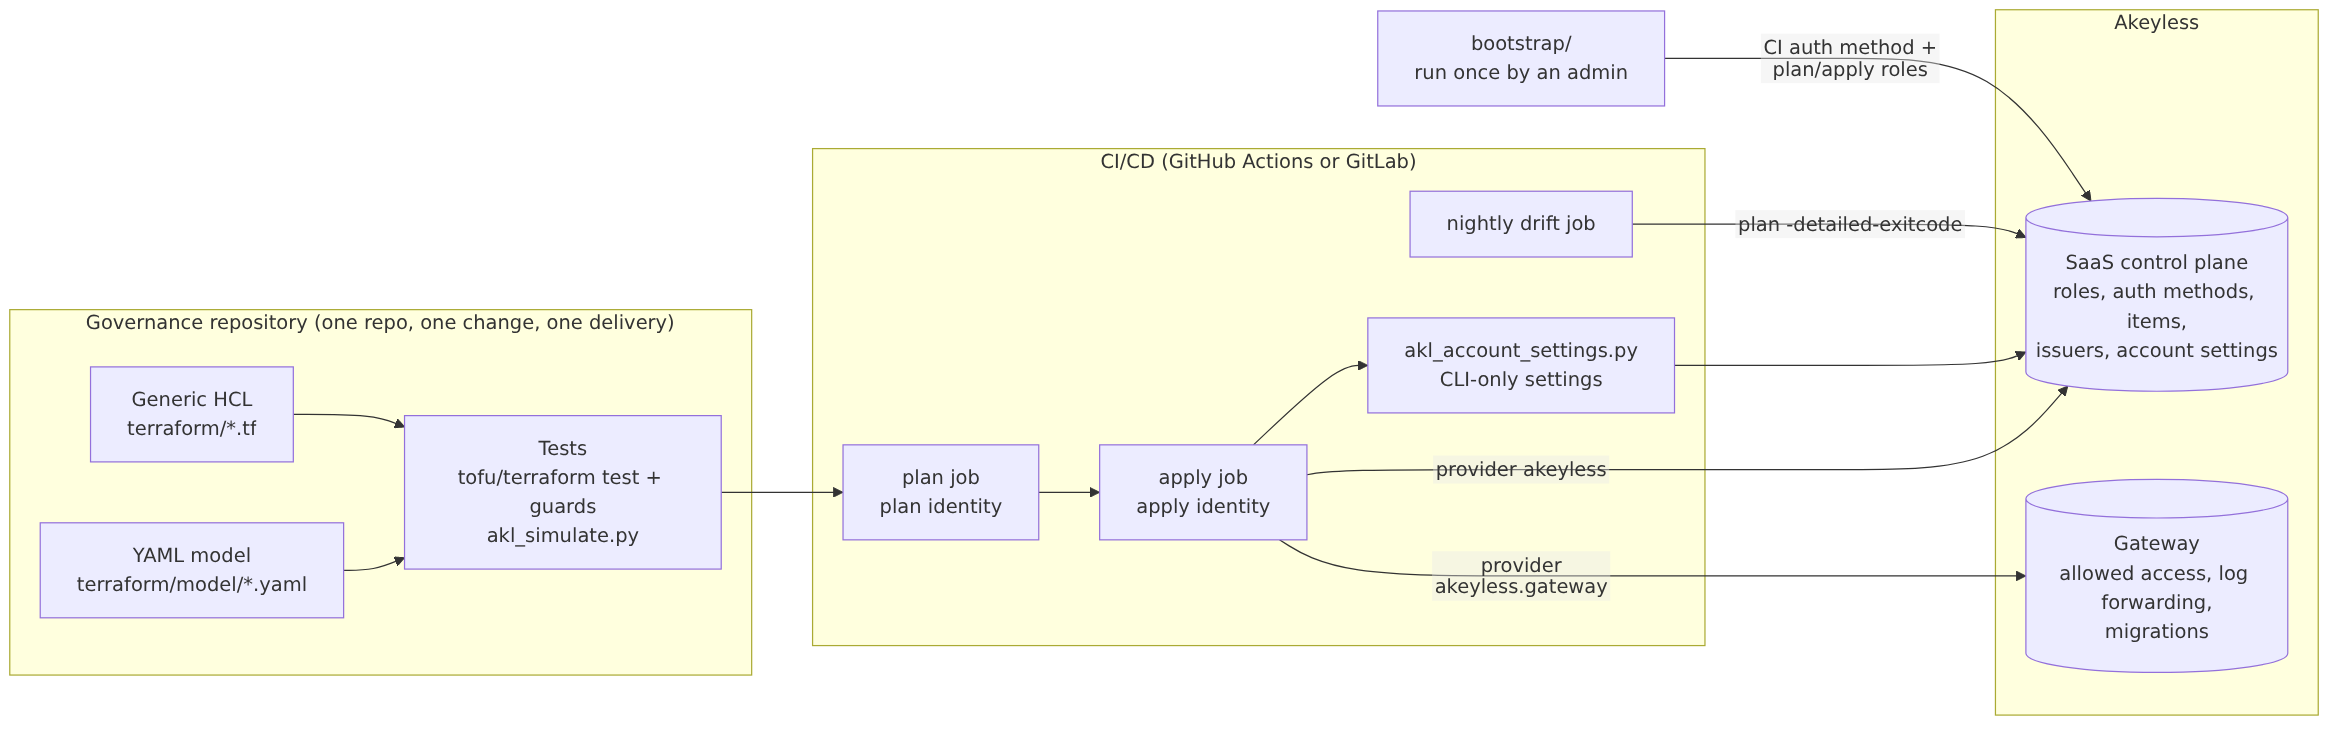
\includegraphics[angle=90,width=\textwidth,height=0.88\textheight]{generated/img/architecture-1.png}
\caption{Diagram from docs/architecture.md}
\end{figure}

\hypertarget{identities}{%
\section{Identities}\label{identities}}

\begin{longtable}[]{@{}
  >{\raggedright\arraybackslash}p{(\columnwidth - 6\tabcolsep) * \real{0.4350}}
  >{\raggedright\arraybackslash}p{(\columnwidth - 6\tabcolsep) * \real{0.1500}}
  >{\raggedright\arraybackslash}p{(\columnwidth - 6\tabcolsep) * \real{0.1510}}
  >{\raggedright\arraybackslash}p{(\columnwidth - 6\tabcolsep) * \real{0.2440}}@{}}
\toprule\noalign{}
\begin{minipage}[b]{\linewidth}\raggedright
Identity
\end{minipage} & \begin{minipage}[b]{\linewidth}\raggedright
Created by
\end{minipage} & \begin{minipage}[b]{\linewidth}\raggedright
Bound to
\end{minipage} & \begin{minipage}[b]{\linewidth}\raggedright
Can
\end{minipage} \\
\midrule\noalign{}
\endhead
\bottomrule\noalign{}
\endlastfoot
Account admin (human) & Akeyless account & - & run \texttt{bootstrap/} once; break-glass \\
CI auth method \texttt{/governance/auth/ci-terraform} (OAuth2/JWT) & \texttt{bootstrap/} & CI OIDC issuer (GitHub or GitLab) & authenticate pipelines, nothing by itself \\
Role \texttt{.../terraform-plan} & \texttt{bootstrap/} & CI auth method, sub-claim = repository & read RBAC/auth config, list items, read \texttt{/pki/*} \\
Role \texttt{.../terraform-apply} & \texttt{bootstrap/} & CI auth method, sub-claims = repository \textbf{and} protected main branch & administer everything it manages (admin-equivalent, because Akeyless forbids granting what you do not hold) \\
Everything in \texttt{terraform/model} & main pipeline & as modelled & as modelled \\
\end{longtable}

The CI identity lives in a separate state (\texttt{bootstrap/}), so the main pipeline can never destroy
its own access.

\hypertarget{what-runs-where}{%
\section{What runs where}\label{what-runs-where}}

\begin{longtable}[]{@{}
  >{\raggedright\arraybackslash}p{(\columnwidth - 4\tabcolsep) * \real{0.1550}}
  >{\raggedright\arraybackslash}p{(\columnwidth - 4\tabcolsep) * \real{0.3750}}
  >{\raggedright\arraybackslash}p{(\columnwidth - 4\tabcolsep) * \real{0.4500}}@{}}
\toprule\noalign{}
\begin{minipage}[b]{\linewidth}\raggedright
Object family
\end{minipage} & \begin{minipage}[b]{\linewidth}\raggedright
API endpoint
\end{minipage} & \begin{minipage}[b]{\linewidth}\raggedright
Terraform provider
\end{minipage} \\
\midrule\noalign{}
\endhead
\bottomrule\noalign{}
\endlastfoot
Roles, rules, associations, auth methods, folders, issuers, keys, custom fields, key policies, event forwarders, account settings & \texttt{https://api.akeyless.io} (or a Gateway\textquotesingle s \texttt{/api/v2}, which proxies the API) & \texttt{akeyless} \\
Gateway allowed access, log forwarding, migrations & the Gateway API (\texttt{https://\textless{}gw\textgreater{}:8000/api/v2} or \texttt{:8081}) & \texttt{akeyless.gateway} (alias) \\
Account settings not exposed by the provider & REST \texttt{/auth} + CLI \texttt{update-account-settings} & - (\texttt{scripts/akl\_account\_settings.py}) \\
\end{longtable}

One Gateway cluster per state: for several clusters, run the same code with one workspace or
var-file per cluster (\texttt{gateway\_api} and \texttt{model/gateway.yaml} differ).

\hypertarget{change-flow}{%
\section{Change flow}\label{change-flow}}

\begin{enumerate}
\def\labelenumi{\arabic{enumi}.}
\tightlist
\item
  Engineer edits YAML (normally only \texttt{model/roles/\textless{}bu\textgreater{}.yaml}) and opens a merge request.
\item
  \texttt{checks}: format, validate, \texttt{terraform\ test} (20+ cases, mocked provider), guard-message proof,
  offline access expectations (\texttt{akl\_simulate.py}), script tests.
\item
  \texttt{plan} with the plan identity; reviewers read the plan (CODEOWNERS: BU + platform).
\item
  Merge -\textgreater{} \texttt{apply} (protected environment, manual approval) -\textgreater{} CLI-only account settings.
\item
  Optional: \texttt{akl\_verify.py} with test personas proves effective access live.
\item
  Nightly \texttt{drift} fails when someone changed Akeyless outside Git; the next apply reverts it
  (role rules are authoritative).
\end{enumerate}
